\documentclass[letterpaper, 11pt]{article}

\usepackage{tikz, listings, comment}
\usepackage[fleqn]{amsmath}
\usepackage[margin=1in]{geometry}
\usepackage{fancyhdr, hyperref, pdfpages}
\usepackage{xcolor}

\definecolor{codegreen}{rgb}{0,0.6,0}
\definecolor{codegray}{rgb}{0.5,0.5,0.5}
\definecolor{codepurple}{rgb}{0.58,0,0.82}
\definecolor{backcolour}{rgb}{0.95,0.95,0.92}

% Disable page numbers
\pagestyle{empty}

%Basic Variables (Modify as required per homework)
\def\class{CompEn 462}
\def\homeworkNumber{1}
\def\date{03.01.2025}
\def\professor{Mark Mahon}

% Define a custom style for listings
\lstdefinestyle{mystyle}{
    backgroundcolor=\color{backcolour},   % Set background color for the code block
    commentstyle=\color{codegreen},       % Set color for comments
    keywordstyle=\color{magenta},         % Set color for keywords
    numberstyle=\tiny\color{codegray},    % Set style for line numbers
    stringstyle=\color{codepurple},       % Set color for strings
    basicstyle=\ttfamily\footnotesize,    % Set basic style for the code
    breakatwhitespace=false,              % Do not break lines at whitespace
    breaklines=true,                      % Allow breaking of lines
    captionpos=b,                         % Set caption position to bottom
    keepspaces=true,                      % Keep spaces in text
    %numbers=left,                         % Display line numbers on the left
    numbersep=5pt,                        % Set distance between line numbers and code
    showspaces=false,                     % Do not show spaces
    showstringspaces=false,               % Do not show spaces in strings
    showtabs=false,                       % Do not show tabs
    tabsize=2                             % Set tab size to 2 spaces
}

\lstset{style=mystyle}

%Code to generate new page for problem
\newcounter{problemId}
\stepcounter{problemId}
\def\newproblem{\clearpage\newpage\noindent{Problem~\arabic{problemId}\stepcounter{problemId}}\hfill\par}

%Custom Section Header Command
\newcommand{\secHeader}[1]{\vspace{2mm} \noindent \textbf{#1:}\vspace{-4mm}}

\begin{document}
%Title page
\hfill
\newline
Name: Justin Ngo
\\PSU ID: jvn5439
\\Professor: \professor
\\Class: \class
\\Date: \date
\\Project : \homeworkNumber

%---------------------ABSTRACT---------------------
\newpage
\secHeader{Abstract}
\vspace{5mm}

This report presents the implementation and analysis of an Orthogonal Frequency Division Multiplexing (OFDM) system and 
covers several key components:

\begin{enumerate}
    \item \textbf{Modulation Schemes}: Different modulation schemes such as BPSK, $\pi$/2-BPSK, QPSK, and 64-QAM are implemented in the 
    \texttt{Modulators.py} file. These schemes are used to convert the input bit stream based off the 8-bit ASCII conversion of the string "WirelessCommunicationSystemsandSecurityJustinNgo"
    into suitable symbols ready for transmission.

    \item \textbf{OFDM Processing}: The \texttt{OFDM.py} file houses all the relevant functions used to produce an OFDM output, and handles the bulk of the processing.
    The OFDM function is responsible for running the serial-to-parallel conversion, Inverse Fast Fourier Transform (IFFT), cyclic prefix insertion, and also graphs the output.

    \item \textbf{Main Execution}: The \texttt{main.py} file generates the bit stream used for processing from the aforementioned phrase and is where the OFDM function is called 
    to run the system for each modulation scheme.

    \item \textbf{Visualization}: A sample of 2 symbols generated from the OFDM system is plotted for visualization and highlights the cyclic prefix and symbol boundaries. 
\end{enumerate}


%---------------------GRAPHS---------------------
\newpage
\secHeader{Generated Waveforms}
\begin{figure}[h!]
    \centering
    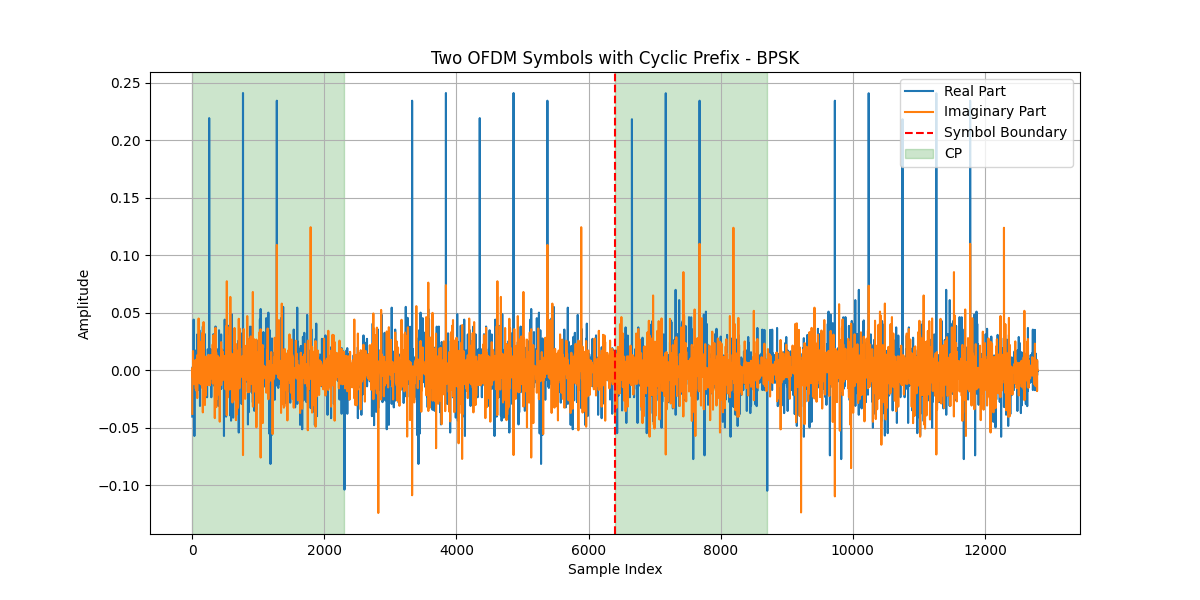
\includegraphics[width=\textwidth,height=4.25in]{BPSK.png}
    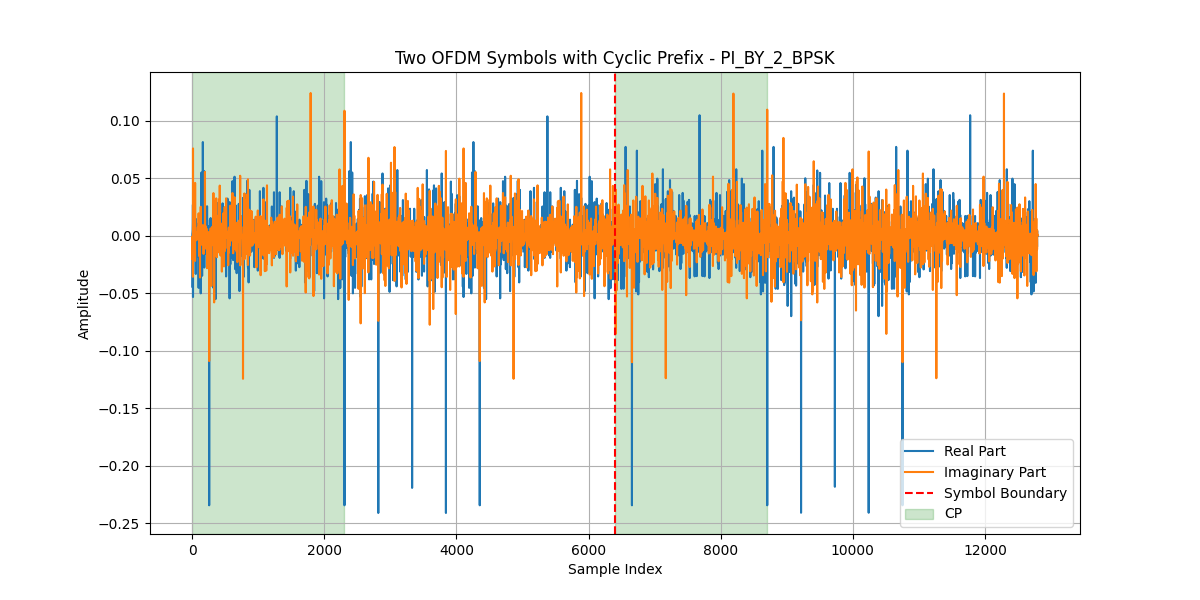
\includegraphics[width=\textwidth,height=4.25in]{PIBPSK.png}
\end{figure}

\newpage
\begin{figure}[h!]
    \centering
    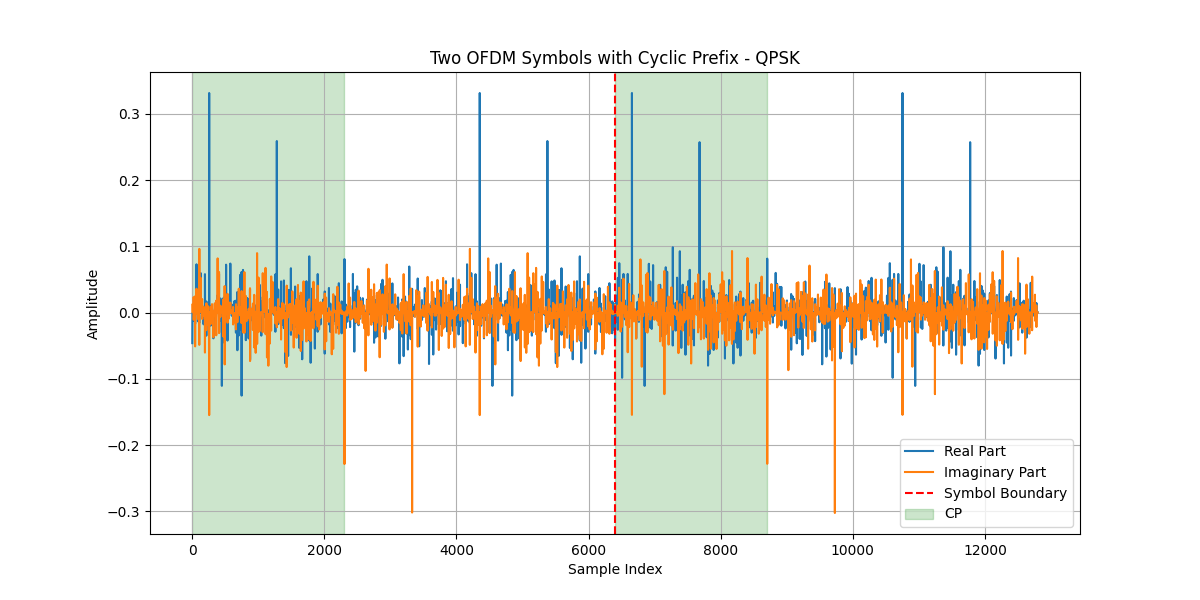
\includegraphics[width=\textwidth,height=4.25in]{QPSK.png}
    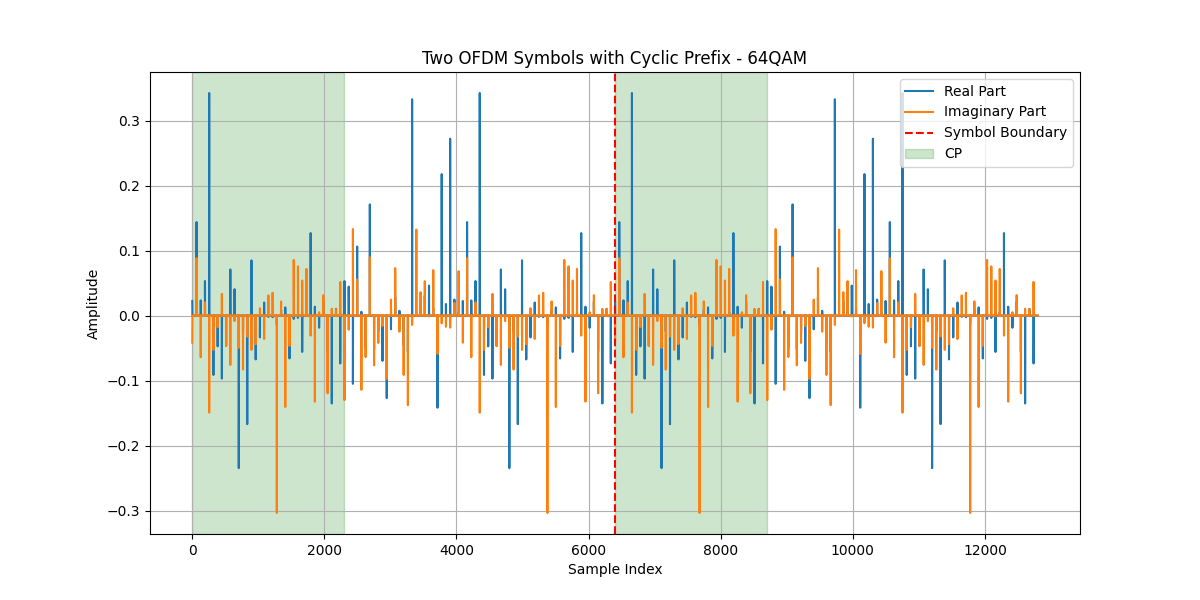
\includegraphics[width=\textwidth,height=4.25in]{64QAM.png}
\end{figure}


%---------------------FLOW DIAGRAM---------------------
\newpage
\secHeader{Flow Diagram}
\vspace{5mm}
\begin{enumerate}
    \item \textbf{Bit Stream Generation}: The input bit stream is generated from the ASCII conversion of the phrase "WirelessCommunicationSystemsandSecurityJustinNgo" 
    and is repeated to ensure a minimum length of 1 slot using the \texttt{64QAM} modulation scheme, since that requires the most bits per symbol.
    \item \textbf{Modulation}: Depending on the modulation scheme passed into the \texttt{OFDM} function, the input bits are mapped to a constellation based off of figure 5.2
    from the book, that was provided in the lecture slides. The formulas I used were approximations of what were provided on the 3GPP TS 38.211 pdf.
    \item \textbf{Serial to Parallel Conversion}: After modulation, the bits are passed into the \\
    \texttt{s2p} function which converts the serial input into a parallel output before running the IFFT
    \item \textbf{IFFT}: The \texttt{IFFT} is run immediately after the bits are reorganized within the \texttt{s2p} function, and is the final output from \texttt{s2p}
    \item \textbf{Cyclic Prefix Insertion}: The 2d array that's returned as the IFFT from \texttt{s2p} is then passed into \texttt{cyc\_pref}, where each symbol 
    is prepended with the last $2034T_c$ of it's output
    \item \textbf{Steps That Weren't Modeled}:
    \begin{enumerate}
        \item \textbf{Parallel to Serial Conversion}: The parallel output of the Prefix Insertions would then be flattened into a serialized output for processing at the DAC
        \item \textbf{DAC}: The DAC would convert the digital signal into an analog signal for transmission
        \item \textbf{RF Modulation}: The analog signal would then be modulated with the carrier frequency to boost the signal before being broadcasted by the antenna
    \end{enumerate}
\end{enumerate}


%---------------------TECHNICAL PROBLEMS---------------------
\newpage
\secHeader{Technical Problems}
\vspace{5mm}
\begin{enumerate}
    \item \textbf{Modulation Schemes}: Had a bit of an issue understanding the math behind the modulation schemes and figuring out how to implement them accurately
    , but wasn't too bad afterwards
    \item \textbf{Cyclic Prefix}: I made an error when I first coded the cyclic prefix insertion, and prematurely flattened the output from the IFFT which caused the code to throw an
    fault and say that the array was inaccessable. Fixed the issue after going over the diagrams again, and only flattened the array after performing the cyclic prefix insertion
\end{enumerate} 
\end{document}